% Overleaf-ready Springer LNCS/LNAI manuscript.
% Main source for the complete IJCKG 2026 Education Track manuscript.
% The framework figure and LNCS class files are included in the Overleaf package.
% Bibliography line spacing is minimally tightened to retain all references within 15 pages.

\documentclass[runningheads]{llncs}

\usepackage[T1]{fontenc}
\usepackage{graphicx}
\usepackage{amsmath}
\usepackage{array}
\usepackage{booktabs}
\usepackage{tabularx}
\usepackage{microtype}
\usepackage{url}
\urlstyle{rm}

\newcommand{\sco}{PSQ-SCO}
\newcommand{\psq}{PersonaShield Quest}
\newcolumntype{Y}{>{\centering\arraybackslash}X}
\newcolumntype{L}{>{\raggedright\arraybackslash}X}
\setlength{\textfloatsep}{9pt plus 2pt minus 2pt}
\setlength{\floatsep}{7pt plus 2pt minus 2pt}
\setlength{\intextsep}{7pt plus 2pt minus 2pt}
\emergencystretch=1.5em

\begin{document}

\title{Ontology-Guided Scenario Control Generation for GenAI in Cybersecurity Serious Game}
\titlerunning{Ontology-Guided Scenario Control for Cybersecurity Education}


%\title{A Scenario Control Ontology for Generative AI in Cybersecurity Education}
%\titlerunning{Scenario Control Ontology for Cybersecurity Education}

\author{Chanphot Wongtaweesup\inst{1} \and
Teeradaj Racharak\inst{2} \and
Watanee Jearanaiwongkul\inst{2} \and
Chutiporn Anutariya\inst{1} \and
Frederic Andres\inst{3}}
\authorrunning{C. Wongtaweesup et al.}

\institute{Asian Institute of Technology (AIT), Pathum Thani, Thailand\\
\email{chanphot.wongtaweesup@ait.asia, chutiporn@ait.ac.th}
\and
Advanced Institute of So-Go-Chi (Convergence Knowledge) Informatics, \\
Tohoku University, Miyagi, Japan\\
\email{racharak@tohoku.ac.jp, watanee@tohoku.ac.jp}
\and
Digital Content and Media Sciences Research Division, \\National Institute of
Informatics, Tokyo, Japan\\
\email{andres@nii.ac.jp}}

\maketitle

\begin{abstract}
Generative artificial intelligence (GenAI) can expand scenario pools for cybersecurity
education; however, fluent outputs may still contain structural errors, omit required
controls, or lack provenance. This paper presents the \psq\ Scenario Control
Ontology (\sco), a task-oriented OWL/RDF knowledge graph that serves as a
pre-generation contract for phishing, smishing, vishing, and legitimate
communication scenarios. Four competency questions specify learner context,
cybersecurity structure, validation rules, and evidence provenance before
generation. We further integrate \sco\ with a serious-game engine and compare four methods -- prompt
only, external text retrieval-augmented generation (RAG), ontology-derived
structured prompting with RAG, and ontology-to-text RAG -- using matched cases across three local language models. The evaluation separately examines ontology functionality, method-invariant scenario conformance, mechanism-specific behavior, evidence traceability, contradiction control, and diversity. Functional tests confirmed
semantic consistency, competency-question coverage, and correct runtime mapping. All experimental conditions 
satisfied the shared executable controls. According to a separately reported secondary operational index, ontology-derived structured prompting achieved the highest mean score for each model,
while typed and verbalized representations produced different repetition
profiles. 
These findings demonstrate that a compact ontology can provide explicit and auditable control, even when baseline prompting already satisfies a constrained game schema.
%The findings show that a compact ontology can add explicit and auditable control even when baseline prompting satisfies a constrained game schema. Its task completeness is limited to the tested questions, conditions, and validation requirements.

\keywords{Cybersecurity Ontology 
\and Knowledge Graphs for Education \and Retrieval-augmented Generation
\and Cybersecurity Education}
\end{abstract}

\section{Introduction}

Artificial intelligence and knowledge graphs increasingly support educational
content and adaptive learning. In cybersecurity education, realistic wording is
not enough: a scenario must place the learner in a relevant role, require an
observable decision, and connect it to feedback and a safe response. Structural
errors or mixed malicious and legitimate cues can make fluent content unusable.

\psq\ is a cybersecurity serious game using simulated email, SMS, and voice
communication. Learners follow a persona path, identify cues, choose a response,
and receive feedback. Malicious cases teach independent verification; legitimate
cases teach calibrated trust. The game logs choices, hints, retries, response
time, and feedback. Its engine therefore needs an executable JSON record with
controls and evidence, not a free-form passage.

Retrieval-augmented generation (RAG) can add contextual examples
\cite{lewis2020}, but an example may not state the role, stage, channel, attack,
safe response, and exclusions that must control the result. Knowledge graphs can
represent these relations and provenance explicitly \cite{hogan2021,pan2024}.
%We therefore test whether a compact application ontology can turn an instructor's
%request into a machine-checkable contract, delivered either as a typed packet or
%as selected ontology records expressed in text.
This paper asks whether a compact scenario-control ontology can make generative cybersecurity scenarios more auditable by exposing learner constraints, cybersecurity concepts, validation rules, safe responses, and provenance before generation. We evaluate this question through ontology tests and a matched four-mode generation comparison. %We do not test learning gains.

The contributions are: \textbf{(1)} a scenario control ontology and four competency
questions linking learner context, cybersecurity structure, safety, and
provenance; \textbf{(2)} an engine comparing typed packets with deterministic
ontology-to-text verbalization; \textbf{(3)} a matched four-condition, three-model
evaluation of function, conformance, grounding, safety, and diversity; and \textbf{(4)} an
instructional workflow linking course intent, scenario review, gameplay evidence,
and content revision. Learner outcomes are not tested.

\section{Related Work}

\subsection{Knowledge Graphs, RAG, and Ontology Guided Generation}

Knowledge graphs support integration, querying, provenance, and explanation
through typed entities and relations \cite{hogan2021}. We use OWL~2, SPARQL~1.1,
SHACL principles, and PROV-O concepts \cite{owl2,provo,sparql,shacl}. RAG supplies
examples to prompts \cite{lewis2020}; KG--LLM research adds symbolic structure
\cite{pan2024}. Evaluation must still separate retrieval relevance, generation
faithfulness, and trace presence \cite{es2024ragas}.

GraphRAG builds graph indexes and summaries \cite{edge2024}; our framework sends
typed values or verbalized records from an OWL/RDF control ontology. Verbalization
requires selection, ordering, and realization \cite{galanis2014}, and fluent text
may still be unfaithful to a graph \cite{hashem2023}. Prior KG-to-text work shows
that representation affects LLM use of retrieved knowledge
\cite{wu2023retrieve}. Here, the text represents a case-specific control subgraph.
Self BLEU and sentence embeddings later measure lexical and semantic repetition
\cite{reimers2019,tevet2021}.

\subsection{Educational Knowledge Graphs and Generative Content}

Educational knowledge graphs support recommendation, explanation, and content
generation. Recent work constructs structured resources
\cite{ain2026ijckg} and grounds a modular RAG tutor \cite{lai2026abel}. Our
ontology instead controls executable fields, safe responses, prohibited concepts,
and provenance before generation, supporting authoring and audit rather than
learner-facing question answering.

\subsection{Cybersecurity Serious Game Scenarios}

Digital games can support learning when instructional design and activity are
aligned \cite{clark2016}. Cybersecurity scenarios should train cue recognition,
independent verification, and safe response. A phishing-game framework connects
interaction and feedback to that task \cite{arachchilage2013}; \sco\ adds MITRE
ATT\&CK and CAPEC links \cite{mitreTaxonomies}.

\subsection{Ontology Engineering and Evaluation}

Ontology engineering requires clear scope, competency questions, and testable
requirements. Test-driven development turns expected answers into positive and
negative tests \cite{keet2016}. We test consistency, query answers, and runtime
mappings to support task completeness, not universal domain completeness.

\section{\sco\ Ontology Requirements and Design}

\subsection{Scope and Modeling Boundary}

The \psq\ Scenario Control Ontology controls the structured information that may
enter the generator: learner and persona constraints, templates, channels,
difficulty, attack structure, evidence, provenance, rules, and engine mappings.
Its scope is scenario control rather than a complete theory of learning.
Objectives, hints, feedback, and difficulty are represented only where they link
a scenario to instructional intent and runtime evidence. An instructor supplies
the practice objective and case controls; the ontology resolves an eligible
template, required concepts, safe response, rules, and source trace. The ontology
is task complete for the four competency questions, four generation conditions,
and validation requirements tested here. It is not a universal model of
cybersecurity or serious games.

\subsection{Competency Questions and Runtime Traceability}

The four competency questions define what the ontology must answer before the
engine creates a scenario. Table~\ref{tab:cq-trace} gives the complete wording of
each question and shows the information retrieved, test result, and engine use. Each
question has one positive and one negative ASK test. The SELECT and ASK queries
were executed with RDFLib~7.6.0.

\begin{table}[!h]
\caption{Competency questions and runtime use.}
\label{tab:cq-trace}
\centering
\scriptsize
\setlength{\tabcolsep}{2.5pt}
\begin{tabularx}{\textwidth}{>{\raggedright\arraybackslash}p{0.55cm}
>{\raggedright\arraybackslash}p{3.45cm}L
>{\raggedright\arraybackslash}p{1.15cm}
>{\raggedright\arraybackslash}p{1.95cm}}
\toprule
\textbf{CQ} & \textbf{Full competency question} & \textbf{Information retrieved and checked} &
\textbf{Test} & \textbf{Engine use}\\
\midrule
CQ1 & Which scenario templates satisfy the learner's current state, requested
stage transition, role, age group, channel, variant, attack type, difficulty, and
retrieval mode? & Match those controls and reject an incompatible template. &
2 rows; 2/2 ASK & Template IDs used to build the prompt.\\
CQ2 & Which cybersecurity attack or legitimate-communication concepts define the
selected scenario template? & Retrieve attack or legitimate concepts,
cues, warning signs or safe indicators, safe response, and ATT\&CK and CAPEC
mappings. & 13 rows; 2/2 ASK & Concepts that the scenario must include or avoid.\\
CQ3 & Which content-quality rules, thresholds, validation decisions, scores, and
violations govern the selected template and generated scenario? & Retrieve eight
active rules and check conditions for acceptance or rejection. & 8 rows; 2/2 ASK
& Rules and decision criteria used by the validator.\\
CQ4 & Which evidence sources, datasets, and provenance records support the
template's attack classification, indicators, and recommended response? & Retrieve
source roles, IDs, datasets, and provenance; reject an incomplete path. & 12 rows;
2/2 ASK & Evidence fields required in the output.\\
\bottomrule
\end{tabularx}
\end{table}

The four answers are used together. CQ1 selects the context. CQ2 defines the
cybersecurity content. CQ3 supplies the quality rules. CQ4 supplies evidence and
provenance. These results populate the learner control, cyber structure, quality
control, and evidence modules shown in Fig.~\ref{fig:framework}.

\subsection{Ontology Profile and Controlled Vocabulary}

The \sco\ graph contains 74 classes, 49 object properties, 39 datatype
properties, and 133 named individuals. The engine groups them into four modules.
Learner control represents role, stage, age, and transition constraints. Cyber
structure represents templates, channels, variants, difficulty, attacks, cues,
and safe responses. Evidence grounding represents source artifacts, retrieval
modes, and provenance. Quality control represents validation rules and decisions.
The runtime profile contains six templates, ten rule records, and twelve evidence
sources; conversion produces 324 short ontology documents. These counts describe
the implemented engine vocabulary, not complete cybersecurity coverage. Creation
method and review status distinguish proposed content from reviewed content.

\subsection{Scenario Control Rules and Enforcement}

CQ3 returns eight active rules from the ten rule records. They cover template
eligibility, attack structure, separation of legitimate content, channel and
persona consistency, evidence, acceptance, and rejection. Some rules cannot be
executed as OWL axioms, so representation and enforcement are separated.
OWL/RDF represents the knowledge, and HermiT checks consistency. SPARQL retrieves
case values and tests valid and invalid patterns. The semantic packet expresses
\texttt{must\_include}, \texttt{must\_exclude}, safe response, and evidence
requirements. Application logic derives labels, retrieves context, and selects
generation context. The runtime validator checks the JSON fields,
message consistency, grounding, safe action, and final decision. SHACL informed
the rule design, although the experiment used the application validator.

Consider an SMS message labeled as malicious. It must use the SMS channel and
smishing concepts. It must contain warning signs and a safe action that verifies
the request through an independent channel. It must not describe the message only
with legitimate indicators. A legitimate SMS message follows the opposite rule.
It needs safe indicators and must not contain malicious attack concepts. OWL
states the concepts and relations, SPARQL selects the relevant values, the packet
guides generation, and the runtime validator checks the completed record.

\section{Ontology-Guided Scenario Generation}

\subsection{Semantic Packet and Reference Specification}

CQ1 to CQ4 assemble a case reference packet containing learner context, channel,
message type, difficulty, attack, safe response, required and prohibited concepts,
evidence, and provenance. It permits varied wording while fixing game controls.
Prompt only is a comparison condition, not ground truth. Direct guidance sends
typed JSON; text guidance sends compact documents with identifiers and relations.

\subsection{Framework Flow and Evaluation Pipeline}

\begin{figure}[!h]
\centering
\IfFileExists{PSQ_SCO_Compact_Framework_Fig1_Updated.png}{%
  \makebox[\textwidth][c]{%
    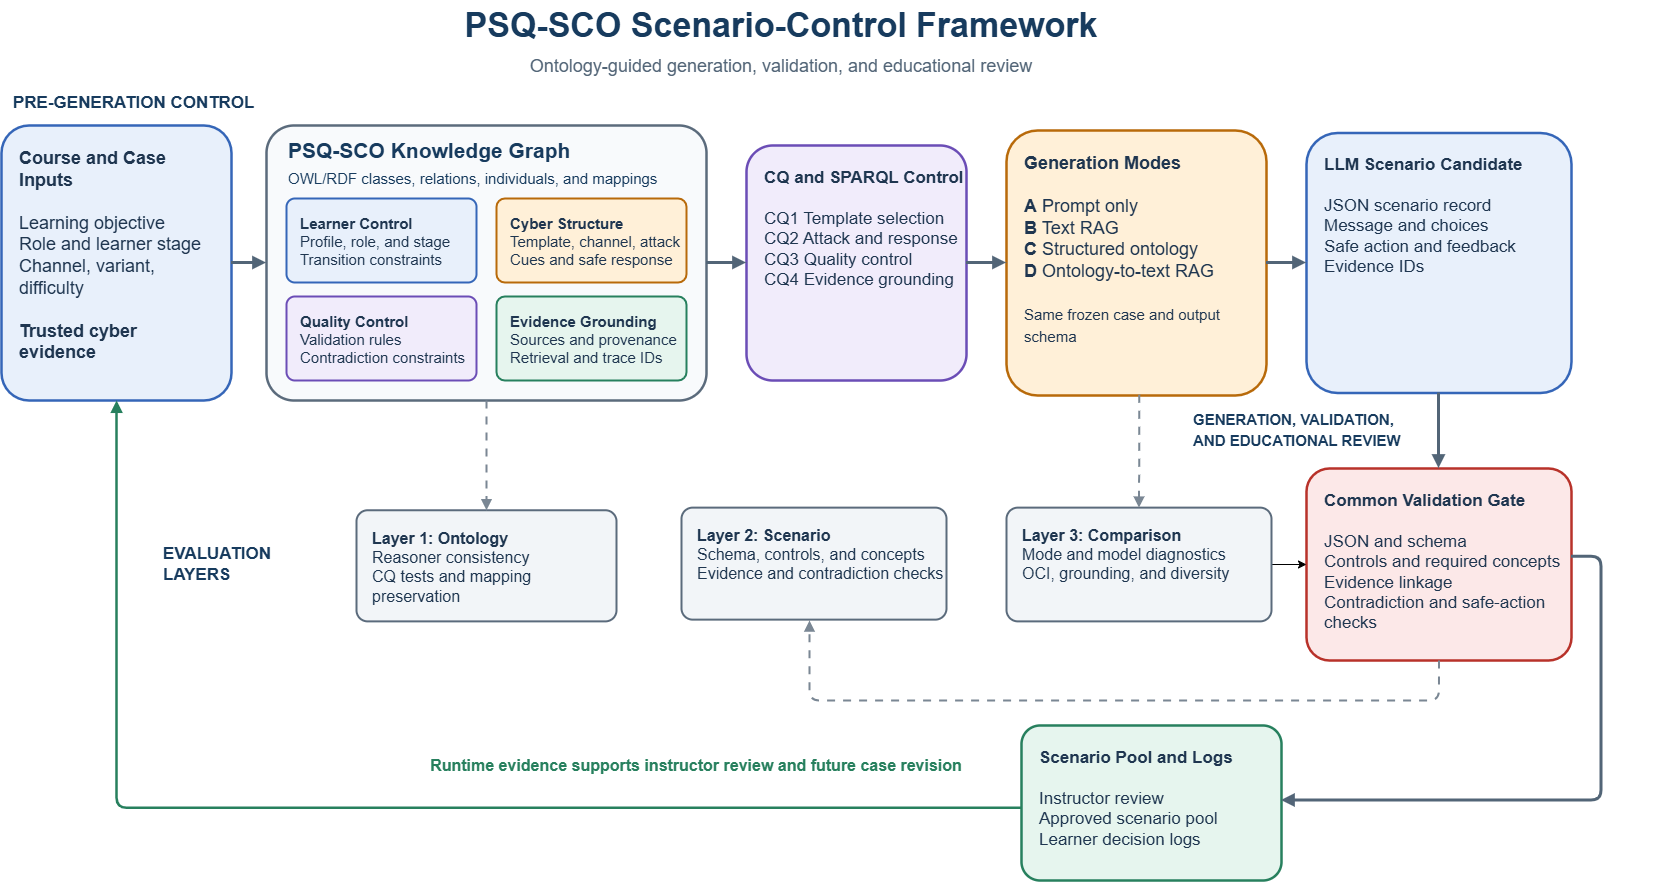
\includegraphics[width=\textwidth]{PSQ_SCO_Compact_Framework_Fig1_Updated.png}}%
}{%
  \fbox{\parbox[c][3.5cm][c]{0.94\textwidth}{\centering
  Upload \texttt{PSQ\_SCO\_Compact\_Framework\_Fig1\_Updated.png}.}}%
}
\caption{PSQ-SCO scenario-control and evaluation framework.}
\label{fig:framework}
\end{figure}

Figure~\ref{fig:framework} presents the PSQ-SCO workflow from instructional input
to reviewed use. Inputs define the objective, learner state, channel, variant,
difficulty, and trusted evidence. The knowledge graph organizes them into learner,
cyber, quality, and evidence modules. CQ1--CQ4 and SPARQL resolve the template,
attack and response, rules, and provenance for the four generation modes, which
produce a common JSON candidate. The gate checks schema, controls, concepts,
evidence, contradictions, and safe action before instructor review and pool
admission. Layers~1--3 evaluate ontology function, scenario conformance, and
mode-model behavior; runtime logs support case revision.

\subsection{Four Generation Modes}

All four modes receive the same frozen case and base JSON schema. They differ in
the additional knowledge supplied to the model.

\paragraph{Mode A: Prompt only.}
The engine sends the case, objective, choice intent, schema, and JSON instructions
without retrieval or ontology records. This is a baseline, not a gold answer.

\paragraph{Mode B: Text RAG.}
ChromaDB retrieves an external example using case controls. Selected filters are
relaxed when no exact match exists, and the model is told not to copy identifiers
or long passages.

\paragraph{Mode C: Structured ontology with RAG.}
The engine combines the same external retrieval with CQ1--CQ4 and serializes the
eligible template, rules, evidence, required and prohibited concepts, and
provenance as a typed packet.

\paragraph{Mode D: Ontology to text RAG.}
The engine combines external retrieval with up to four of 324 verbalized ontology
records selected by a deterministic lexical ranker. The records represent a
template, rule, evidence source, and graph trace. They enter as text and are not
embedded or stored in Chroma. This mode is ontology to text, not ontology
embedding. All modes share the output schema and post-generation gate; only the
information supplied before generation changes.

Table~\ref{tab:conditions} separates the information given to each mode from the
common validation gate. This makes the proposed mechanism explicit and prevents a
retrieval source, an ontology representation, and a validation result from being
treated as the same construct. The expected mechanism is a design rationale, not
an observed result.

\begin{table}[!htbp]
\caption{Generation conditions and mechanisms.}
\label{tab:conditions}
\centering
\fontsize{7.2}{7.8}\selectfont
\setlength{\tabcolsep}{1.1pt}
\renewcommand{\arraystretch}{0.98}
\begin{tabularx}{0.97\textwidth}{>{\raggedright\arraybackslash}p{1.75cm}LLLL}
\toprule
\textbf{Field} & \textbf{A: Prompt} & \textbf{B: Text RAG} &
\textbf{C: Structured ontology} & \textbf{D: Ontology to text}\\
\midrule
Prompt input & Case, objective, choices, and schema. & Base prompt plus a retrieved
example. & Base prompt plus a typed semantic packet and any retrieved example. &
Base prompt plus selected ontology documents and any retrieved example.\\
Retrieval source & None. & External Chroma corpus. & External Chroma corpus, when
available, plus SPARQL results from the ontology KG. & External Chroma corpus,
when available, plus the 324-record ontology-text corpus.\\
Ontology use & None. & None. & CQ1--CQ4 select packet values. & Packet anchors and
case terms rank verbalized ontology records.\\
Format & JSON instructions. & Natural-language example. & Typed JSON
fields. & Fixed-format text records.\\
Constraints & Schema and case values. & Base constraints plus example. & Required
and prohibited concepts, rule, response, and evidence fields. & The same controls
expressed in selected text records.\\
Validation & Common post-generation gate. & Common post-generation gate. & Common
post-generation gate. & Common post-generation gate.\\
Expected mechanism & No-retrieval baseline. & Add contextual realism. & Make typed
obligations explicit. & Supply ontology controls through text-compatible RAG.\\
\bottomrule
\end{tabularx}
\end{table}

\paragraph{Selected subgraph.}
Mode D builds a case-conditioned record set. Let $\mathcal{T}_c$ denote the case
terms, $A$
the packet anchor identifiers, and $d$ a verbalized record. Records are ranked by
\begin{equation}
s(d)=2\!\sum_{q\in \mathcal{T}_c}\!I(q\in d)+8I(d\text{ references }A)
 +2I(\mathrm{type}(d)\in\{T,R,E\}),
\end{equation}
where $I(\cdot)$ is the indicator function and $T$, $R$, and $E$ denote template,
rule, and evidence records. Ties are
resolved by record identifier. The selector reserves the highest-ranked record
of each type and then fills open positions with unseen records. The result is a
small, case-specific control subgraph rather than the complete ontology.

\paragraph{Graph walk and verbalization.}
An optional deterministic greedy walk starts from at most five packet anchors. It
scores query-term matches in each relation, target, label, definition, and RDF
type, adds one point for a known control record, orders ties by property and
target, and stops at depth two. All four document slots were occupied by the
selected template, rule, evidence, and trace records, so no walk document entered
the prompts. The experiment therefore tests lexical selection, not a graph walk.

Each selected record uses a fixed verbalization template:
\begin{center}\small
\texttt{ID; record type; label; definition; selected relations; generation use.}
\end{center}
A template states its channel, message type, cues, and safe response; a rule states
its condition and prohibited combination. This favors auditability, although
selection, order, and wording can affect faithfulness \cite{galanis2014,hashem2023}.

\paragraph{Frozen experiment.}
The same 120 cases are used for each mode and model. Thirty channel--variant--role
groups combine three difficulty anchors with one balanced repetition. Every case
fixes role, stage pair, age, channel, variant, difficulty, attack, and safe
response. Qwen2.5 7B, Qwen3 8B, and Mistral 7B through Ollama produce
$120\times4\times3=1{,}440$ live outputs with no fallback records.

External retrieval used a cosine HNSW ChromaDB index containing 28,728 records
from 23 files. No custom embedding was supplied; Chroma documents
\texttt{all-MiniLM-L6-v2} as its default \cite{chromaDefault}. The run did not
store the Chroma version, model revision, or hash, so this is the expected rather
than fully frozen retrieval identity. The model is general purpose, while ontology
records are semi-structured. Mode D uses lexical ontology-record selection and
makes no ontology-embedding claim; results are conditional on the selector,
ordering, and verbalization.

\subsection{Worked Scenario Example}

An implemented case gives a beginner IT-support persona an urgent, malicious SMS.
The learner must detect spoofing and verify the link, domain, and sender through an
approved channel. Prompt only sends the case and schema; Text RAG adds an example;
structured ontology uses CQ1 for the template, CQ2 for cues and safe response, CQ3
for rules, and CQ4 for sources; ontology to text verbalizes those records. The game
record contains three choices, a hint, feedback, and independent verification as
the correct action. The evaluator checks controls, cues, and context identifiers.

For course authoring, the instructor defines the objective and safe behavior; the
ontology resolves permitted content, and the engine creates playable email, SMS,
and voice variants under one contract. This supports content planning and later
transfer assessment. The experiment tests control preservation, and every final
scenario still requires instructional review.

\section{Evaluation Design}

The evaluation asks whether the ontology answers its competency questions and
preserves runtime mappings, whether four input representations preserve the same
case controls and evidence path, and how their safety decisions and repetition
differ. A rule-based specification fixes role, age group, stage, channel, variant,
difficulty, attack type, safe response, and required concepts. Frozen identifiers
link all 1,440 live-model records. Prompt output is a baseline, not ground truth;
the measures evaluate the artifact and generated content, not learner outcomes.

\subsection{Layer 1: Ontology Validation}

HermiT checks consistency and unsatisfiable classes \cite{hermit}. One positive
and one negative SPARQL ASK test evaluate each competency question. Mapping tests
check whether controls survive conversion between engine and ontology records:

\begin{equation}
\mathrm{CQPassRate}=\frac{\mathrm{passed\ CQ\ tests}}
{\mathrm{total\ CQ\ tests}},
\quad
\mathrm{MappingPassRate}=\frac{\mathrm{passed\ mapping\ tests}}
{\mathrm{total\ mapping\ tests}} .
\end{equation}

Runtime compatibility counts records preserved after conversion.

\subsection{Layer 2: Scenario Validation}

Each output is compared with its structured case specification rather than one
reference passage. Different wording is therefore allowed when the same game
controls are preserved.

\paragraph{JSON validity and schema completeness.}
JSON validity requires an inspectable scenario object. Schema completeness checks
\texttt{scenario\_id}, channel, variant, choices, correct action, difficulty, and
warning signs or safe indicators. Evidence fields are measured separately, so
parseable JSON can still fail the game schema.

\paragraph{Control adherence.}
Control adherence checks eight case controls: role, age group, the stage pair,
channel, variant, difficulty, attack type, and safe response. It is the fraction
of expected controls that match:

\begin{equation}
\mathrm{ControlAdherence}=\frac{\mathrm{number\ of\ matched\ control\ fields}}
{\mathrm{number\ of\ expected\ control\ fields}},
\end{equation}

A score of 1 means that every checked control matches. The measure concerns
instruction following, not writing fluency.

\paragraph{Concept precision, recall, and F1.}
For case $c$, $R_c$ contains the required channel, variant, attack or legitimate
type, role, cues, verification behavior, and defensive action. The same set is
used for every mode; Prompt is not the reference. A controlled-vocabulary matcher
forms generated set $G_c$ and match set $M_c=G_c\cap R_c$:

\begin{equation}
P=\frac{|M_c|}{|G_c|},\qquad
R=\frac{|M_c|}{|R_c|},\qquad
F1=\frac{2PR}{P+R}.
\end{equation}

Matched and missing lists are saved for every row. F1 measures closed-label
concept coverage.

\paragraph{Evidence grounding.}
$G$ is the fraction of six required source/provenance fields present. For output
$c$, $L_c$ contains its declared source, dataset, provenance-record, and ordered
context links; $V_c\subseteq L_c$ contains those resolving to the correct frozen
local record. Thus $T_c=|V_c|/|L_c|$, or not applicable if $L_c$ is empty.
Neither $G$ nor $T$ proves claim--source support, which remains unevaluated;
retrieval relevance and generation faithfulness are distinct \cite{es2024ragas}.

\paragraph{Secondary mechanism diagnostics.}
The method-conditioned required-concept scores may include packet terms and
provenance available only to a given mode. They explain mechanism exposure rather
than cross-mode accuracy. A separate ontology-scope diagnostic counts implemented
channel, attack, cue, response, evidence, and non-contradiction checks in the
trace; it is a rule audit, not OWL entailment or ontology-embedding accuracy.

Composite indices can summarize multidimensional diagnostics, but their
interpretation depends on weighting and aggregation; nominal weights may not
equal empirical influence, so components and weight sensitivity should be reported
\cite{greco2019composite,becker2017weights}. Accordingly, we treat the component
metrics as primary and report the equal-weight operational index only as a
secondary descriptive summary:
\begin{equation}
\mathrm{OCI}_{\mathrm{eq}}=
\frac{J+A+F_{\mathrm{req}}+G+(1-E)}{5},
\label{eq:operational-index}
\end{equation}
where $J$, $A$, $F_{\mathrm{req}}$, $G$, and $E$ denote JSON validity, control
adherence, method-conditioned concept F1, provenance completeness, and
contradiction rate. Equal nominal weights express the absence of a validated
differential model, not objective fairness. OCI$_{\mathrm{eq}}$ is secondary,
descriptive, uncalibrated, and neither a quality percentage, threshold, nor
learner-effect measure. Sensitivity compares the earlier engine-priority weights.

\paragraph{Contradiction and technical decision.}
Contradiction rate is the share of records with a prohibited error, such as mixed
malicious and legitimate cues or an unsafe action. A noncompensatory gate rejects
invalid JSON or contradictions, requests missing controls, and otherwise accepts
the row for human review. Acceptance is not classroom approval.

\paragraph{Diversity.}
Two collection metrics check repetition. Embedding diversity subtracts mean
pairwise cosine similarity from 1:

\begin{equation}
\mathrm{EmbeddingDiversity}=1-\operatorname*{mean}_{i<j}
\cos(E_i,E_j),
\end{equation}

It uses \texttt{sentence-transformers/all-MiniLM-L6-v2} within each 120-case model
and mode set, then averages across models. Larger values mean less similarity.
Self BLEU compares each scenario with the rest of its set:

\begin{equation}
\mathrm{SelfBLEU}=\frac{1}{N}\sum_i \mathrm{BLEU}(x_i,X_{-i}).
\end{equation}

Higher embedding diversity and lower Self BLEU indicate less repetition
\cite{reimers2019,tevet2021}. Normalized title and ordered-choice repetition is the
share of patterns occurring more than once.

\paragraph{Treatment delivery and efficiency.}
Full exposure means that a row received every context component specified by its
condition, although a RAG mode may return no external text. Incomplete telemetry
precludes a speed comparison.

\subsection{Layer 3: Method and Model Comparison}

Each mode contributes 360 rows: 120 matched cases generated by three models.
Cochran's $Q$ compares matched binary gate decisions \cite{cochran1950}. Schema,
control, and common-case concept scores are validation results. The secondary
equal-weight operational index in Eq.~\ref{eq:operational-index} and the diversity measures describe differences
between implemented representations; they are not general quality rankings.

\section{Results}

\subsection{Layer 1 Results: Ontology Functional Validation}

HermiT found \sco\ consistent with no unsatisfiable classes. All eight positive
and negative ASK controls passed, and engine--ontology mapping preserved all 1,440
records.

\paragraph{Competency-question results.}
The SELECT queries returned the following answers. \textbf{CQ1} selected two
English SMS templates for an HR learner aged 22--35 progressing from Beginner
Introductory to Developing: the fake ``Urgent bank verification link'' and the
legitimate ``Expected internal reminder.'' \textbf{CQ2} returned 13 bindings for
SMS smishing, ATT\&CK T1566.003, CAPEC-164, credential harvesting, fear, urgency,
three red flags, independent verification, and reporting. \textbf{CQ3} returned
eight eligibility, consistency, evidence, separation, acceptance, and rejection
rules; the candidate was marked for review with quality .92, confidence .88, and
no violation. \textbf{CQ4} returned 12 bindings connecting the advanced voice
template's classification, red flags, and end-call-and-verify response to ATT\&CK
T1566.004, CAPEC-164, a peer-reviewed source, an IRS transcript, and a provenance
record. Together, these results support task completeness for the tested questions
and runtime interface, not universal cybersecurity coverage.

Layer 1 establishes logical consistency, discrimination of expected and
prohibited cases by CQ1--CQ4, and preservation of selected controls in runtime
mappings. It validates task-level ontology function, not generated text or learner
outcomes.

\subsection{Layer 2 Results: Common Scenario Conformance}
\label{subsection:diag}

All 1,440 outputs were valid JSON, complete for the game schema, and exact on the
eight frozen controls. Common-case precision, recall, and F1 were 1.000 in every
condition. Here, ``common case'' means the same method-invariant concept set was
checked for every output: channel, variant, attack or legitimate type, learner
role, required cues, verification behavior, and safe response. Precision 1.000
means that no conflicting concept from this shared vocabulary was counted; recall
1.000 means that every required shared concept was detected; therefore F1 was
also 1.000. These values show exact preservation of the frozen labels, not perfect
wording, realism, provenance, pedagogical quality, or learning effectiveness.

The gate accepted 1,439 records for human review and returned one for
regeneration; decision rates did not differ (Cochran's $Q=3.00$, $p=.392$).
Layer 2 therefore confirms that the common gate was executable for all modes. Its
ceiling cannot distinguish the representations, which are compared in Layer 3.

\subsection{Layer 3 Results: Method and Model Comparison}

Layer 3 evaluates method-conditioned control exposure and model stability.
Table~\ref{tab:method} reports diagnostics that complement the Layer 2 measures.

\begin{table}[!h]
\caption{Mean method diagnostics across three models ($n=360$ per condition).}
\label{tab:method}
\centering
\fontsize{6.25}{6.9}\selectfont
\setlength{\tabcolsep}{1.05pt}
\begin{tabular}{@{}>{\raggedright\arraybackslash}p{1.72cm}rrrrrrrrrr@{}}
\toprule
\textbf{Condition} & \textbf{$J\uparrow$} & \textbf{$A\uparrow$} &
\textbf{$P\uparrow$} & \textbf{$R\uparrow$} & \textbf{$F1_{\rm req}\uparrow$} &
\textbf{$G\uparrow$} & \textbf{$T\uparrow$} &
\shortstack{\textbf{Ont.}\\\textbf{scope}$\uparrow$} &
\textbf{$E\downarrow$} & \textbf{OCI$_{\rm eq}\uparrow$}\\
\midrule
Prompt only            & \textbf{1.000} & \textbf{1.000} & .382 & .795 & .512 & .481 & -- & .400 & \textbf{.000} & .799\\
Text RAG               & \textbf{1.000} & \textbf{1.000} & .318 & .779 & .448 & .782 & .928 & .400 & \textbf{.000} & .846\\
Structured ontology    & \textbf{1.000} & \textbf{1.000} & \textbf{.508} & .596 & \textbf{.545} & \textbf{1.000} & \textbf{.996} & \textbf{.900} & \textbf{.000} & \textbf{.909}\\
Ontology to text       & \textbf{1.000} & \textbf{1.000} & .270 & \textbf{.809} & .399 & \textbf{1.000} & .968 & .865 & .003 & .879\\
\bottomrule
\end{tabular}
\par\vspace{2pt}
\begin{minipage}{0.97\textwidth}
\fontsize{7.0}{7.6}\selectfont
\emph{Symbols:} $J$, JSON validity; $A$, control adherence; $P$ and $R$, method-conditioned required-concept precision and recall; $F1_{\rm req}$, their harmonic mean; $G$, required provenance-field presence; $T$, resolution of declared links to frozen local records; Ont. scope, ontology trace/control coverage; $E$, contradiction rate. $T$ is conditional on declared links (applicable $n$: 0, 226, 360, and 360); ``--'' means not applicable. Component metrics are primary; OCI$_{\rm eq}$ is the secondary descriptive summary in Eq.~\ref{eq:operational-index}.
\end{minipage}
\end{table}

Structured ontology has the highest method-conditioned $P$ (.508) and $F1_{\rm req}$ (.545); ontology to text has the highest $R$ (.809). $G$ is complete for C and D. Conditional mean $T$ is .996 for C, .968 for D, and .928 for B; A declares no links. $E$ is zero for A--C and .003 for D. External text was returned for 226 Text-RAG, 221 structured-ontology, and 242 ontology-to-text rows; every ontology row retains identifiers.

OCI$_{\rm eq}$ orders the tested conditions C, D, B, A with means .909, .879, .846, and .799. Legacy weights give the same condition and within-model ranks.

Table~\ref{tab:model-index} is a secondary stability view: C is highest for each model, conditional on these components rather than universal quality.

\begin{table}[!h]
\caption{Secondary OCI$_{\rm eq}$ by model and condition.}
\label{tab:model-index}
\centering
\scriptsize
\setlength{\tabcolsep}{5.0pt}
\begin{tabular}{@{}>{\raggedright\arraybackslash}p{2.65cm}rrrr@{}}
\toprule
\textbf{Model} & \textbf{A: Prompt} & \textbf{B: Text RAG} &
\textbf{C: Structured} & \textbf{D: Ontology text}\\
\midrule
Mistral 7B & .7754 & .8446 & \textbf{.9019} & .8788\\
Qwen2.5 7B & .8100 & .8502 & \textbf{.9035} & .8782\\
Qwen3 8B & .8101 & .8434 & \textbf{.9214} & .8808\\
\midrule
Mean       & .7985 & .8461 & \textbf{.9089} & .8793\\
\bottomrule
\end{tabular}
\end{table}

In 10,000 deterministic weight samples, C ranks first in 100.0\%; pairwise stability is 82.8\% for B versus A, 81.9\% for D versus A, and 80.7\% for D versus B. Components therefore remain primary.

\subsubsection{Five matched diagnostic cases.}
Table~\ref{tab:five-cases} compares all four stored outputs for each deterministically selected case/model pair. The supplement gives verbatim excerpts, concept lists, $G$, $T$, $E$, and safe-action results.

\begin{table}[!h]
\caption{Deterministically selected matched-case diagnostics.}
\label{tab:five-cases}
\centering
\fontsize{7.0}{7.6}\selectfont
\setlength{\tabcolsep}{2.5pt}
\begin{tabularx}{0.97\textwidth}{@{}>{\raggedright\arraybackslash}p{1.7cm}>{\raggedright\arraybackslash}p{2.15cm}X@{}}
\toprule
\textbf{Selection} & \textbf{Case/model} & \textbf{Matched observation}\\
\midrule
Median pair & 053/Mistral 7B & All modes pass $E$ and safe action; pair OCI$_{\rm eq}$ is nearest the complete-pair median.\\
Contradiction & 023/Qwen3 8B & Mode D has $E=1$ and requires regeneration; matched A--C have $E=0$.\\
No ext. RAG & 002/Mistral 7B & Mode B retrieved no context, so $T$ is not applicable; its shared gate passed.\\
Legitimate & 070/Qwen2.5 7B & All modes retain the legitimate label and safe workflow without contradiction.\\
P/R trade-off & 064/Qwen3 8B & Mode D exposes $P=0.171$ and $R=1.000$, the largest disclosed gap.\\
\bottomrule
\end{tabularx}
\end{table}

\paragraph{Diversity and repetition.}

\begin{table}[!h]
\caption{Diversity diagnostics.}
\label{tab:diversity}
\centering
\scriptsize
\setlength{\tabcolsep}{4pt}
\begin{tabular}{@{}>{\raggedright\arraybackslash}p{3.3cm}rrrr@{}}
\toprule
\textbf{Condition} & \textbf{Emb. div. $\uparrow$} &
\textbf{Self BLEU $\downarrow$} & \textbf{Title rep. $\downarrow$} &
\textbf{Choice rep. $\downarrow$}\\
\midrule
Prompt only & .343 & .885 & .769 & .572\\
Text RAG & .375 & .811 & .700 & .681\\
Structured ontology & \textbf{.388} & \textbf{.791} & .642 & \textbf{.458}\\
Ontology to text & .376 & .806 & \textbf{.589} & .703\\
\bottomrule
\end{tabular}
\end{table}

Table~\ref{tab:diversity} reports repetition within each 360-scenario condition.
Structured ontology has the highest embedding diversity (.388), lowest Self BLEU
(.791), and lowest repeated-choice rate (.458); its scenarios therefore vary more
in semantic content, wording, and choice structure. Ontology to text has the
lowest repeated-title rate (.589) but highest repeated-choice rate (.703), meaning
that titles vary while answer-option structures recur. Prompt only has the lowest
semantic diversity and highest Self BLEU, consistent with greater reuse of meaning
and wording. Semantic, lexical, title, and choice diversity therefore describe
different properties and do not support one universal ranking.

No output contained invalid JSON, an incomplete schema, a wrong channel or attack
label, or an unsafe action. Nonuniform telemetry prevents an efficiency comparison.

\section{Discussion}

\subsection{What the Ontology Adds}

The central finding is control observability. Text RAG can add an example but may
return no context or typed template, response, rule, and evidence identifiers.
Structured ontology supplies those fields directly; ontology to text supplies
documents whose effect depends on selection, order, and verbalization. Structured
ontology has the highest method-conditioned precision, F1, and traceability and leads three diversity measures; ontology to text has the
lowest title repetition. Mode D remains bounded by its four-document lexical
selector and does not test ontology embeddings. Prompt only also reached the
conformance ceiling (Section~\ref{subsection:diag}); ontology guidance is therefore
not shown to be necessary for this schema. Rather, structured guidance provides
greater provenance, typed control exposure, and auditability. Its first-place OCI$_{\rm eq}$ rank is descriptive, not universal.

\subsection{Educational Meaning of Scenario Control}

Before play, role, stage, channel, and difficulty define the practice context;
cues and safe responses define the decision to be learned. During play, choices,
hints, feedback, and retries make the process observable. Instructors can trace an
objective to its template and safe action, review admission to the pool, and use
logged decisions to revise examples or progression. This supports educational
authoring and assessment readiness, but does not demonstrate learning improvement.

\subsection{Instructional Deployment Workflow}

The framework separates instructional decisions from language generation. An
instructor specifies the objective, learner stage, channel, variant, difficulty,
and safe response. CQ1 selects templates, CQ2 supplies cybersecurity concepts and
exclusions, CQ3 supplies validation rules, and CQ4 attaches provenance. A mode
then generates the message, choices, action, hint, feedback, and evidence fields.
The common gate checks the candidate, but instructor approval is still required
before admission to the scenario pool. During play, the scenario identifier links
choices, hints, retries, and response time to the template and objective. These
logs support revision of examples, feedback, or progression, forming a traceable
cycle without assigning pedagogical authority to the language model.

\subsection{Threats to Validity}

Frozen identifiers hold controls constant and every row came from a live call,
but one output per cell cannot estimate decoding variation. Some assigned RAG rows
received no external text. The closed-label oracle tests control preservation, not
realism, paraphrase quality, or learning. Link resolution verifies paths, not claim support; source similarity lacks frozen relevance
judgments. OCI$_{\rm eq}$ is uncalibrated, although nominal ranks and 10,000-weight sensitivity are reported. Diversity uses one embedding model, and English email, SMS, and voice
cases do not cover every culture, organization, or attack family.

\section{Limitations, Ethics, and Future Work}

\sco\ controls phishing, smishing, vishing, and legitimate communication, not all
cybersecurity or learning theory. Task completeness covers only the tested
questions, conditions, and rules. Evidence fields and local paths support auditing but do not
prove source quality or claim support; experts must review scenarios and mappings. One run and schema-safe repairs limit decoding and content-stability inference.

\paragraph{Ethics and data governance.}
The cases use fictional personas and no learner records. The engine uses inert
links, checks safe actions, and retains evidence. Source bias, outdated guidance,
licensing, privacy, and dual use remain risks. Deployment should minimize data,
control access, set retention limits, and obtain consent for learner studies
\cite{pardo2014}.

Future work will repeat cells under fixed decoding, complete telemetry, and a
frozen embedding artifact, while preserving retrieval ranks, judgments, and
claim-source links. Graph-walk and ontology-embedding ablations will be separate.
Expert and classroom studies will assess realism, decisions, feedback, transfer,
and retention. Further experiments will compare stronger and lightweight
open-source models with paid models and test other educational domains requiring
structured constraints and traceable evidence.

\section{Conclusion}

This study presents a task-oriented ontology, four executable CQs, two ontology
delivery mechanisms, and a matched four-mode evaluation. Reasoning, ASK, and
mapping tests confirm that the control contract works for the declared task, and
all modes passed the common executable checks. Structured ontology has the highest method-conditioned precision, F1, and mean traceability; ontology to text has the highest recall. Secondary OCI$_{\rm eq}$ is .799, .846, .909, and .879 for A--D, with C highest for each model under both nominal weightings. Because common conformance reached ceiling performance (Section~\ref{subsection:diag}), these results indicate mechanism exposure, not superior scenario quality in general. Ontology to text remains useful for text-only interfaces and
reduced title repetition. The findings establish educational content control and
auditability, not learning gains; expert and classroom studies remain necessary.

\begin{credits}
\subsubsection{\discintname}
The authors declare no competing interests.
\subsubsection{Generative AI Use}
The authors used \mbox{ChatGPT 5.6} for grammar and readability, reviewed all
suggestions, and retain responsibility for the manuscript.
\end{credits}

\begingroup
\makeatletter
\let\psqoldthebibliography\thebibliography
\renewcommand{\thebibliography}[1]{%
  \psqoldthebibliography{#1}%
  \fontsize{7.8}{8.2}\selectfont
  \setlength{\itemsep}{0pt}%
  \setlength{\parsep}{0pt}%
}
\makeatother
\bibliographystyle{splncs04}
\bibliography{references}
\endgroup

\end{document}
